\documentclass[tikz,border=4pt]{standalone}
\usepackage{ctex}
\usepackage{amsmath}
\usepackage{pgfplots}
\pgfplotsset{compat=1.18}
\begin{document}
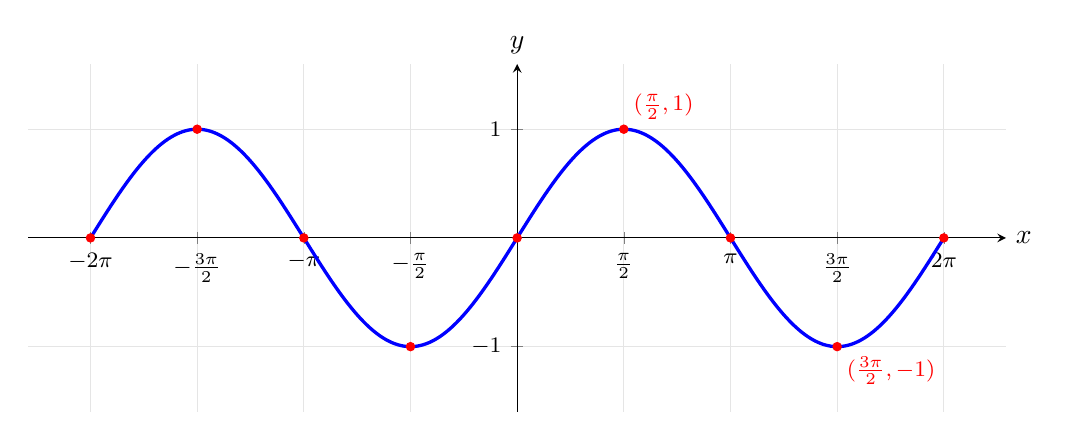
\begin{tikzpicture}
\begin{axis}[
    axis lines=middle,
    xmin=-7.2, xmax=7.2,
    ymin=-1.6, ymax=1.6,
    width=14cm, height=6cm,
    xlabel={$x$}, ylabel={$y$},
    xlabel style={right}, ylabel style={above},
    samples=400,
    grid=both,
    grid style={gray!20},
    xtick={-6.2832,-4.7124,-3.1416,-1.5708,0,1.5708,3.1416,4.7124,6.2832},
    xticklabels={$-2\pi$,$-\tfrac{3\pi}{2}$,$-\pi$,$-\tfrac{\pi}{2}$,$0$,$\tfrac{\pi}{2}$,$\pi$,$\tfrac{3\pi}{2}$,$2\pi$},
    ytick={-1,1},
    tick label style={font=\footnotesize},
]
\addplot[blue, very thick, domain=-6.2832:6.2832] {sin(deg(x))};
\addplot[only marks, mark=*, mark size=1.5pt, red] coordinates {
  (0,0) (1.5708,1) (3.1416,0) (4.7124,-1) (6.2832,0)
  (-1.5708,-1) (-3.1416,0) (-4.7124,1) (-6.2832,0)
};
\node[above right, font=\footnotesize, red] at (axis cs:1.5708,1) {$(\tfrac{\pi}{2},1)$};
\node[below right, font=\footnotesize, red] at (axis cs:4.7124,-1) {$(\tfrac{3\pi}{2},-1)$};
\end{axis}
\end{tikzpicture}
\end{document}
